\documentclass[tikz,border=4pt]{standalone}
\usepackage[T1]{fontenc}
\usepackage{lmodern}
\renewcommand{\familydefault}{\sfdefault}
\usetikzlibrary{shapes.geometric,positioning,arrows.meta,calc,fit,backgrounds,decorations.pathreplacing}
\tikzset{
  node distance=6mm,
  every node/.style={font=\footnotesize,align=center,execute at begin node={\hyphenpenalty=10000\relax}},
  base/.style={draw=gray!60,fill=gray!12,minimum height=7mm,inner sep=2pt},
  term/.style={base,rounded corners=3.5mm,text width=30mm},
  proc/.style={base,text width=32mm},
  err/.style={base,text width=30mm,fill=gray!22},
  io/.style={base,trapezium,trapezium left angle=72,trapezium right angle=108,trapezium stretches=true,text width=28mm},
  dec/.style={base,diamond,aspect=2.4,text width=27mm,inner sep=0pt},
  % predefined process: a call to another procedure
  sub/.style={proc,inner xsep=3mm,path picture={
    \draw[gray!60] ([xshift=1.5mm]path picture bounding box.north west)--([xshift=1.5mm]path picture bounding box.south west)
                   ([xshift=-1.5mm]path picture bounding box.north east)--([xshift=-1.5mm]path picture bounding box.south east);}},
  go/.style={-{Stealth[length=2mm]},draw=gray!55!black},
  lab/.style={font=\scriptsize,fill=white,inner sep=1pt},
  frame/.style={draw=gray!60,dashed,rounded corners=2mm,inner sep=3mm},
  % memory diagrams
  cell/.style={draw=gray!60,fill=gray!12,minimum height=7mm,inner sep=1pt,font=\scriptsize},
  hot/.style={cell,fill=gray!35},
  note/.style={font=\scriptsize,text=gray!30!black},
}

\begin{document}
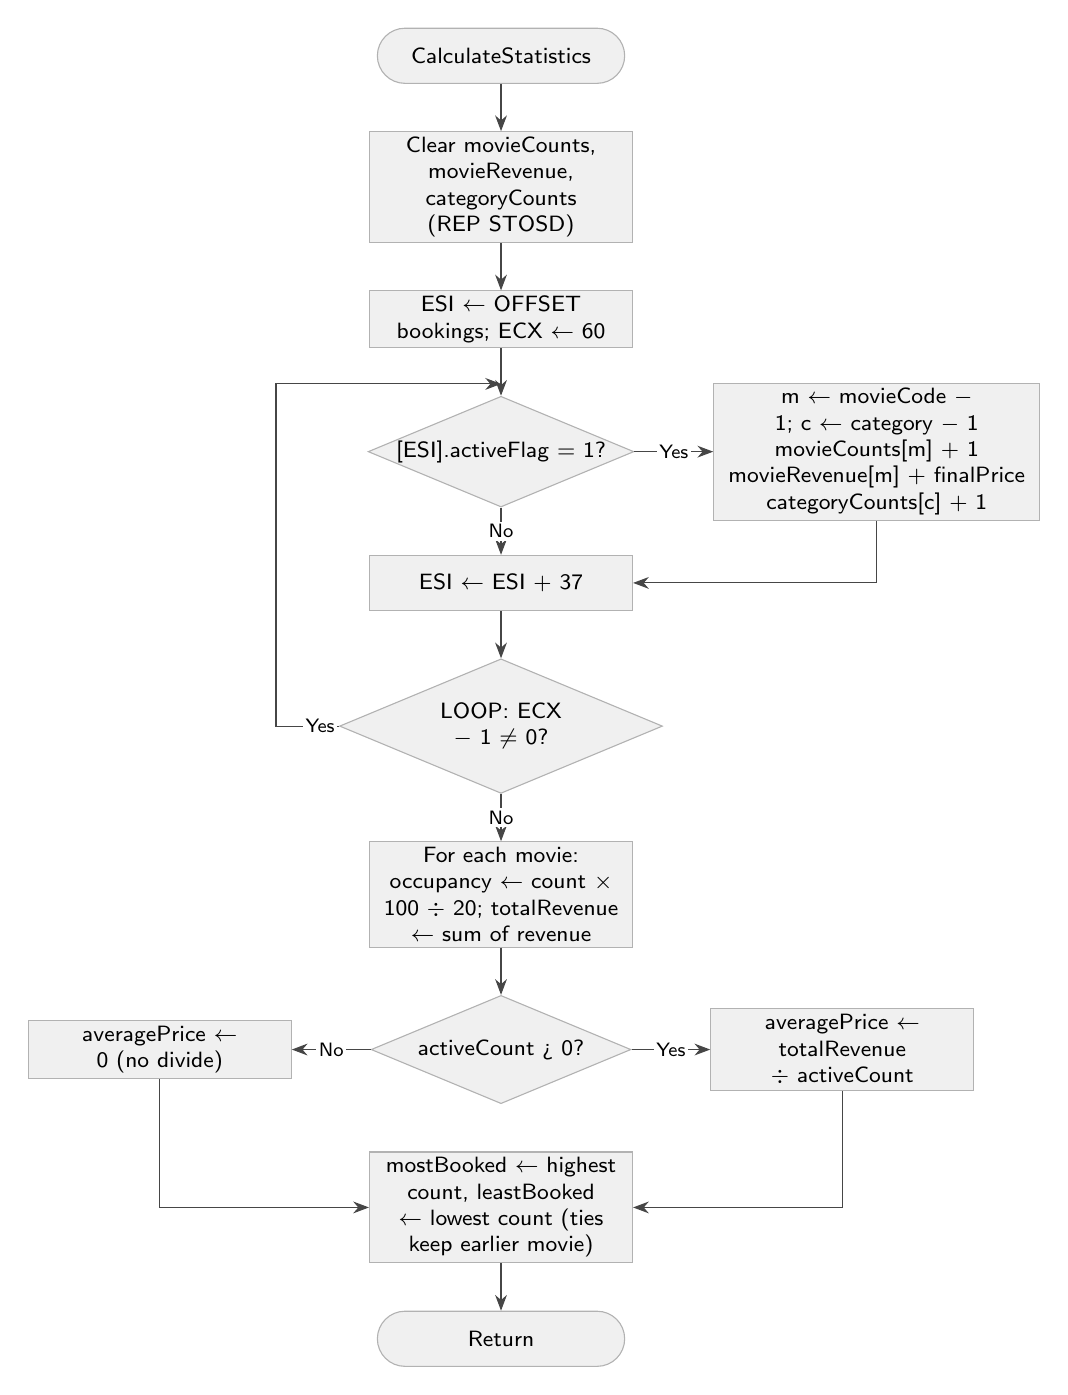
\begin{tikzpicture}
\node[term] (s) {CalculateStatistics};
\node[proc,below=of s] (c) {Clear movieCounts, movieRevenue, categoryCounts (REP STOSD)};
\node[proc,below=of c] (i) {ESI $\leftarrow$ OFFSET bookings; ECX $\leftarrow$ 60};
\node[dec,below=of i] (d1) {[ESI].activeFlag = 1?};
\node[proc,right=10mm of d1,text width=40mm] (u) {m $\leftarrow$ movieCode $-$ 1; c $\leftarrow$ category $-$ 1\\ movieCounts[m] + 1\\ movieRevenue[m] + finalPrice\\ categoryCounts[c] + 1};
\node[proc,below=of d1] (n) {ESI $\leftarrow$ ESI + 37};
\node[dec,below=of n] (l) {LOOP: ECX $-$ 1 $\neq$ 0?};
\node[proc,below=of l] (o) {For each movie: occupancy $\leftarrow$ count $\times$ 100 $\div$ 20; totalRevenue $\leftarrow$ sum of revenue};
\node[dec,below=of o] (d2) {activeCount > 0?};
\node[proc,right=10mm of d2] (av) {averagePrice $\leftarrow$ totalRevenue $\div$ activeCount};
\node[proc,left=10mm of d2] (z) {averagePrice $\leftarrow$ 0 (no divide)};
\node[proc,below=of d2] (m) {mostBooked $\leftarrow$ highest count, leastBooked $\leftarrow$ lowest count (ties keep earlier movie)};
\node[term,below=of m] (e) {Return};
\draw[go] (s)--(c);
\draw[go] (c)--(i);
\draw[go] (i)--(d1);
\draw[go] (d1)--node[lab]{Yes}(u);
\draw[go] (u)|-(n.east);
\draw[go] (d1)--node[lab]{No}(n);
\draw[go] (n)--(l);
\draw[go] (l.west)--node[lab,pos=.3]{Yes}++(-8mm,0)|-([yshift=1.5mm]d1.north);
\draw[go] (l)--node[lab]{No}(o);
\draw[go] (o)--(d2);
\draw[go] (d2)--node[lab]{Yes}(av);
\draw[go] (d2)--node[lab]{No}(z);
\draw[go] (av)|-(m.east);
\draw[go] (z)|-(m.west);
\draw[go] (m)--(e);
\end{tikzpicture}
\end{document}
